% Assisted-Living Smart Home - Vortragsfolien (ca. 11 min)
% Kompilieren: pdflatex praesentation.tex  (zweimal fuer Refs)
\documentclass[aspectratio=169,11pt]{beamer}

\usetheme{metropolis}
% Hinweis: babel-german ist in dieser Umgebung nicht installiert. Auf einem System
% mit texlive-lang-german kann fuer korrekte Silbentrennung
% \usepackage[ngerman]{babel} ergaenzt werden.
\usepackage[utf8]{inputenc}
\usepackage[T1]{fontenc}
\usepackage{tikz}
\usetikzlibrary{positioning,arrows.meta,shapes.geometric,calc,backgrounds,fit}
\usepackage{booktabs}
\usepackage{array}

\metroset{numbering=fraction,progressbar=foot,sectionpage=progressbar,block=fill}

\definecolor{mDarkTeal}{HTML}{0E4D64}
\definecolor{mLightBrown}{HTML}{EB811B}
\definecolor{accentBlue}{HTML}{1F6FB2}
\definecolor{accentGreen}{HTML}{2E8B57}
\definecolor{accentRed}{HTML}{C0392B}
\definecolor{softGray}{HTML}{ECEFF1}
\setbeamercolor{frametitle}{bg=mDarkTeal}

\tikzset{
  node distance=8mm and 12mm,
  dev/.style={draw=accentBlue, thick, rounded corners=2pt, fill=accentBlue!8,
              font=\scriptsize, align=center, minimum height=7mm, minimum width=15mm},
  broker/.style={draw=mLightBrown, very thick, fill=mLightBrown!12, font=\small\bfseries,
                 align=center, minimum height=12mm, minimum width=30mm, rounded corners=3pt},
  hub/.style={draw=accentGreen, very thick, fill=accentGreen!10, font=\small\bfseries,
              align=center, minimum height=14mm, minimum width=28mm, rounded corners=3pt},
  web/.style={draw=mDarkTeal, thick, fill=mDarkTeal!8, font=\scriptsize, align=center,
              minimum height=10mm, minimum width=24mm, rounded corners=3pt},
  flow/.style={-{Stealth[length=2.5mm]}, thick, accentBlue},
  flowg/.style={-{Stealth[length=2.5mm]}, thick, accentGreen},
  lbl/.style={font=\tiny\itshape, fill=white, inner sep=1pt},
}

\title{Smart Home f\"ur betreutes Wohnen}
\subtitle{Ein verteilter, ereignisgesteuerter Demonstrator auf MQTT-Basis}
\date{Heterogeneous Computing, SS 2026}
\author{Joel Deffner}

\begin{document}

\maketitle

% ============================================================
\begin{frame}{Was gebaut wurde und warum}
  \textbf{Szenario:} Wohnung im betreuten Wohnen. Sensorik soll Pflegekr\"afte bei
  kritischen Situationen alarmieren (Sturz/SOS, Herd vergessen, n\"achtliches Verlassen des Bettes).

  \vspace{1.2em}
  \textbf{Aufgabe:} Aus Recherche zu Smart-Home-Architekturen zentrale Anforderungen
  ableiten und einen prototypischen Demonstrator aus \emph{mehreren kommunizierenden
  Komponenten} umsetzen. Physische Hardware wird softwareseitig simuliert.

  \vspace{1.2em}
  \begin{columns}[T]
    \column{0.5\textwidth}
      \textbf{Stack}
      \begin{itemize}
        \item Docker + Eclipse Mosquitto (MQTT-Broker)
        \item TypeScript / Node, je Komponente ein Prozess
        \item Web-Konsole (Express + SSE)
      \end{itemize}
    \column{0.5\textwidth}
      \textbf{Kernidee}
      \begin{itemize}
        \item Kein Ger\"at spricht ein anderes direkt an
        \item Alles l\"auft als Pub/Sub \"uber den Broker
        \item Logik rein lokal (Edge), keine Cloud
      \end{itemize}
  \end{columns}
\end{frame}

% ============================================================
\begin{frame}{Von der Recherche zu den Anforderungen}
  \textbf{Beobachtungen aus bestehenden Plattformen} (Home Assistant, openHAB, ioBroker):
  zentral / dezentral / hybrid; \textbf{MQTT} und CoAP auf Kommunikationsebene;
  Zigbee, Z-Wave, Thread, Wi-Fi, BLE auf Funkebene; \textbf{Matter} als IP-basierte
  Interoperabilit\"atsschicht; Trend zur Trennung von \textbf{Cloud} und \textbf{Edge}.

  \vspace{1em}
  \begin{block}{Abgeleitete Kernanforderungen}
    \begin{columns}[T]
      \column{0.5\textwidth}
        \begin{itemize}
          \item Verteilung
          \item Skalierbarkeit
          \item Fehlertoleranz
        \end{itemize}
      \column{0.5\textwidth}
        \begin{itemize}
          \item Lose Kopplung
          \item Heterogenit\"at der Ger\"ate
          \item Erweiterbarkeit
        \end{itemize}
    \end{columns}
  \end{block}
  \vspace{0.3em}
  {\small Diese sechs Anforderungen sind der rote Faden f\"ur jede Entwurfsentscheidung im Folgenden.}
\end{frame}

% ============================================================
\begin{frame}{Architektur: Ger\"at $\rightarrow$ Broker $\rightarrow$ Hub}
  \begin{center}
  \resizebox{0.78\textwidth}{!}{%
  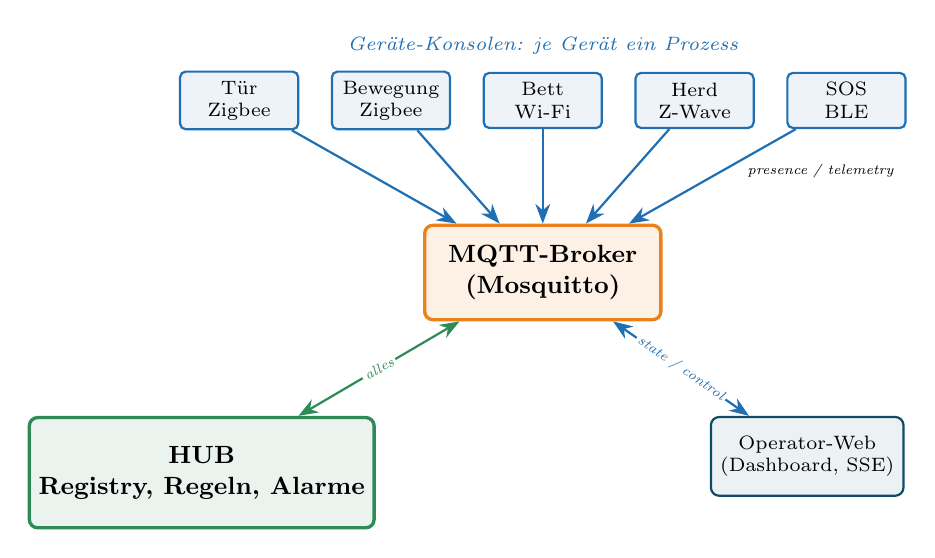
\begin{tikzpicture}
    \node[dev] (d1) {T\"ur\\Zigbee};
    \node[dev, right=4mm of d1] (d2) {Bewegung\\Zigbee};
    \node[dev, right=4mm of d2] (d3) {Bett\\Wi-Fi};
    \node[dev, right=4mm of d3] (d4) {Herd\\Z-Wave};
    \node[dev, right=4mm of d4] (d5) {SOS\\BLE};
    \node[above=1mm of d3, font=\scriptsize\itshape, text=accentBlue] {Ger\"ate-Konsolen: je Ger\"at ein Prozess};

    \node[broker, below=12mm of d3] (br) {MQTT-Broker\\(Mosquitto)};

    \node[hub, below left=12mm and 6mm of br] (hub) {HUB\\Registry, Regeln, Alarme};
    \node[web, below right=12mm and 6mm of br] (web) {Operator-Web\\(Dashboard, SSE)};

    \foreach \d in {d1,d2,d3,d4,d5} {
      \draw[flow] (\d) -- (br);
    }
    \node[lbl] at ($(d5)!0.5!(br) + (1.6,0.2)$) {presence / telemetry};

    \draw[flowg, {Stealth[length=2.5mm]}-{Stealth[length=2.5mm]}] (br) -- (hub)
      node[lbl, midway, sloped] {alles};
    \draw[flow, {Stealth[length=2.5mm]}-{Stealth[length=2.5mm]}] (br) -- (web)
      node[lbl, midway, sloped] {state / control};
  \end{tikzpicture}}
  \end{center}

  \vspace{0.4em}
  {\footnotesize Vier Prozessarten, gekoppelt \emph{nur} \"uber Topics. F\"allt eine Komponente aus,
  laufen die anderen weiter; retained Messages und persistierte Dateien erm\"oglichen Re-Sync beim Neustart.}
\end{frame}

% ============================================================
\begin{frame}{Kommunikationsmodell: Publish/Subscribe \"uber Topics}
  Hierarchische Topics, Wildcards (\texttt{+}, \texttt{\#}) erm\"oglichen Ger\"ateerkennung
  \emph{ohne} zentrale Konfiguration. QoS\,1 (mindestens einmal).

  \vspace{0.6em}
  \begin{center}
  \footnotesize
  \begin{tabular}{@{}l l l@{}}
    \toprule
    \textbf{Topic} & \textbf{Inhalt} & \textbf{Eigenschaft} \\
    \midrule
    \texttt{registry/<id>}            & Ger\"ate-Datensatz + Status    & retained \\
    \texttt{devices/<id>/presence}    & online / offline               & retained, \textbf{Last-Will} \\
    \texttt{devices/<id>/telemetry}   & Messwert + Akku + Signal       & fl\"uchtig \\
    \texttt{devices/<id>/command}     & Steuerbefehl an Ger\"at        & fl\"uchtig \\
    \texttt{pairing/<serial>}         & Pairing-Anzeige (neues Ger\"at)& retained, Last-Will \\
    \texttt{alarms/<id>}              & aktiver Alarm                  & retained \\
    \texttt{rooms/<id>} \& \texttt{hub/status} & R\"aume, Tag/Nacht-Fenster & retained \\
    \bottomrule
  \end{tabular}
  \end{center}

  \vspace{0.6em}
  {\small \textbf{Ein einziger Vertrag:} JSON \"uber MQTT, typisiert in einer geteilten
  Datei (\texttt{src/shared/types.ts}). Hub und Sensor k\"onnen nicht auseinanderlaufen.}
\end{frame}

% ============================================================
\section{Nicht-triviale Konzepte}

% ------------------------------------------------------------
\begin{frame}{Konzept 1: Fehlertoleranz aus dem Protokoll}
  Fehlererkennung ist \emph{nicht} aufwendige Anwendungslogik, sondern ergibt sich aus
  zwei MQTT-Mechanismen.

  \vspace{0.8em}
  \begin{columns}[T]
    \column{0.52\textwidth}
      \textbf{Last-Will (LWT)}\\
      Beim Verbinden hinterlegt jedes Ger\"at beim Broker eine Nachricht
      \texttt{presence = offline} (retained). Stirbt der Prozess (Absturz, Fenster zu,
      Netz weg), \emph{publiziert der Broker sie automatisch}.

      \vspace{0.8em}
      \textbf{Retained State}\\
      Registry, R\"aume und Status sind retained. Eine sp\"ater startende Komponente sieht
      sofort den kompletten Bestand, ohne jemand abfragen zu m\"ussen.

    \column{0.46\textwidth}
      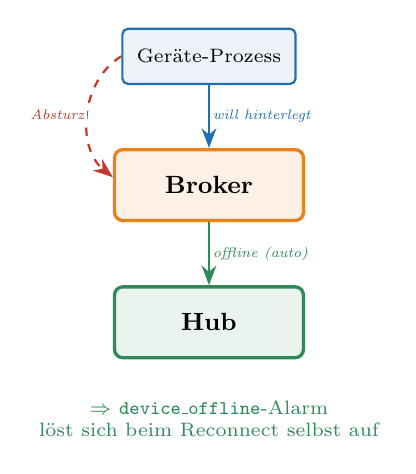
\begin{tikzpicture}[node distance=6mm]
        \node[dev, minimum width=22mm] (s) {Ger\"ate-Prozess};
        \node[broker, minimum width=24mm, minimum height=9mm, below=8mm of s] (b) {Broker};
        \node[hub, minimum width=24mm, minimum height=9mm, below=8mm of b] (h) {Hub};
        \draw[flow] (s) -- node[lbl,right]{will hinterlegt} (b);
        \draw[flow, accentRed, dashed] (s.west) to[bend right=55]
            node[lbl, left]{\textcolor{accentRed}{Absturz}} ($(b.west)+(0,1mm)$);
        \draw[flowg] (b) -- node[lbl,right]{offline (auto)} (h);
        \node[font=\scriptsize, below=4mm of h, align=center, text=accentGreen]
          {$\Rightarrow$ \texttt{device\_offline}-Alarm\\ l\"ost sich beim Reconnect selbst auf};
      \end{tikzpicture}
  \end{columns}
  \vspace{0.4em}
  {\small Zus\"atzlich: Auto-Reconnect alle 2\,s; fehlerhafte Nachrichten werden geloggt, nicht weitergereicht.}
\end{frame}

% ------------------------------------------------------------
\begin{frame}{Konzept 2: Onboarding wie bei echter Hardware}
  Ein neues Ger\"at bootet \textbf{unprovisioniert}, genau wie ab Werk. Es hat noch keine
  ID und keinen Raum, sondern nur eine Werks-Identit\"at (Serien-Nr. + Setup-PIN).

  \vspace{0.8em}
  \begin{center}
  \resizebox{\textwidth}{!}{%
  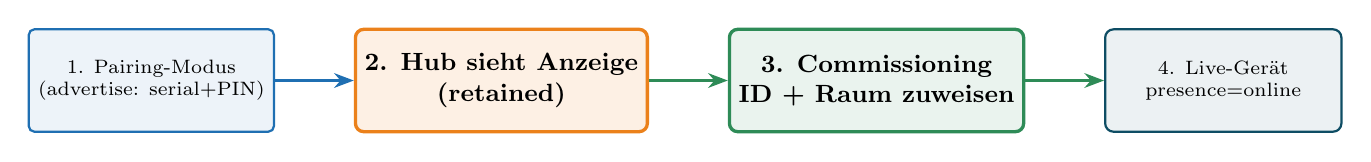
\begin{tikzpicture}[node distance=5mm]
    \node[dev, minimum width=30mm, minimum height=13mm] (a) {1. Pairing-Modus\\(advertise: serial+PIN)};
    \node[broker, minimum width=26mm, minimum height=13mm, right=10mm of a] (b) {2. Hub sieht Anzeige\\(retained)};
    \node[hub, minimum width=30mm, minimum height=13mm, right=10mm of b] (c) {3. Commissioning\\ID + Raum zuweisen};
    \node[web, minimum width=30mm, minimum height=13mm, right=10mm of c] (d) {4. Live-Ger\"at\\presence=online};
    \draw[flow] (a) -- (b);
    \draw[flowg] (b) -- (c);
    \draw[flowg] (c) -- (d);
  \end{tikzpicture}}
  \end{center}

  \vspace{0.6em}
  \begin{itemize}
    \item Commissioning entweder direkt in der Konsole \emph{oder} per Klick im Web
          (,,Ger\"ate, die auf Pairing warten``); Raumwahl per ,,QR-Scan`` des Raumcodes.
    \item Abbruch vor dem Commissioning r\"aumt die Pairing-Anzeige automatisch wieder ab (Last-Will).
    \item Bewusst angelehnt an Zigbee/Z-Wave-Inclusion bzw. Matter-Setup-Codes.
  \end{itemize}
\end{frame}

% ------------------------------------------------------------
\begin{frame}{Konzept 3: Regel- und Alarm-Engine}
  Der Hub trennt sauber: \textbf{Regeln} erkennen Situationen, die \textbf{Alarm-Engine}
  verwaltet deren Lebenszyklus.

  \vspace{0.6em}
  \begin{columns}[T]
    \column{0.5\textwidth}
      \textbf{Regeln}\\
      Pro Ger\"at kleiner Zustand (wann Herd an, wann Bett verlassen, letzte Bewegung im Raum).
      Eine Situation wird \emph{einmal} beim Eintreten erhoben und \emph{einmal} beim Ende
      gel\"oscht, kein Dauerfeuer.

      \vspace{0.6em}
      \textbf{Latchender SOS-Alarm}\\
      Der Notfallknopf modelliert echtes Verhalten: Loslassen l\"oscht den Alarm \emph{nicht}.
      Er bleibt kritisch, bis eine Pflegekraft aktiv quittiert.

    \column{0.5\textwidth}
      \footnotesize
      \begin{tabular}{@{}l l@{}}
        \toprule
        \textbf{Regel} & \textbf{Schwere} \\
        \midrule
        \texttt{sos\_pressed} & \textcolor{accentRed}{kritisch} \\
        \texttt{stove\_on\_no\_motion} & \textcolor{accentRed}{kritisch} \\
        \texttt{bed\_left\_at\_night} & \textcolor{accentRed}{kritisch} \\
        \texttt{door\_open\_no\_motion} & \textcolor{mLightBrown}{Warnung} \\
        \texttt{device\_offline} & \textcolor{mLightBrown}{Warnung (auto)} \\
        \bottomrule
      \end{tabular}
      \vspace{0.6em}

      {\scriptsize Alarme sind retained und \emph{dedupliziert}: dasselbe Problem erzeugt
      keinen zweiten Alarm. Schwellen sind per Env-Var konfigurierbar (kurz f\"ur Demos).}
  \end{columns}
\end{frame}

% ------------------------------------------------------------
\begin{frame}{Heterogenit\"at hinter einem Datenmodell}
  F\"unf Ger\"atetypen \"uber vier Funkstandards, jeweils mit realistischem Datenblatt
  (Hersteller, Modell, Akku\,\%, RSSI, Firmware) und doch ein gemeinsames Nachrichtenformat.

  \vspace{0.6em}
  \begin{center}
  \footnotesize
  \begin{tabular}{@{}l l l l@{}}
    \toprule
    \textbf{Typ} & \textbf{Produkt (sim.)} & \textbf{Transport} & \textbf{Energie} \\
    \midrule
    T\"ur / Kontakt  & Aqara DW-S100        & Zigbee & Batterie \\
    Bewegung (PIR)   & Philips Hue SML-002  & Zigbee & Batterie \\
    Bettbelegung     & Emfit QS-Care        & Wi-Fi  & Netz \\
    Herdw\"achter    & Inirv Guard-Z        & Z-Wave & Netz \\
    SOS-Anh\"anger   & CareTech SOS-Pendant & BLE    & Batterie \\
    \bottomrule
  \end{tabular}
  \end{center}

  % \vspace{0.6em}
  % {\small Der Funkstandard ist Metadatum, das Verhalten realistisch simuliert (Akku entl\"adt,
  % Signal schwankt, Herd k\"uhlt ab). Konzeptionell dieselbe Idee wie \textbf{Matter}:
  % eine gemeinsame Schicht \"uber heterogenen Funktechniken.}
\end{frame}

% ============================================================
\section{Anforderungen \& Demo}

% ------------------------------------------------------------
\begin{frame}{Wie die Kernanforderungen konkret gel\"ost sind}
  \scriptsize
  \begin{tabular}{@{}p{0.22\textwidth} p{0.74\textwidth}@{}}
    \toprule
    \textbf{Anforderung} & \textbf{Umsetzung im Prototyp} \\
    \midrule
    \textbf{Verteilung} & Eigenst\"andige Prozesse (Hub, Sensoren, Web), gekoppelt nur \"uber den Broker; Logik lokal/verteilt. \\[2pt]
    \textbf{Skalierbarkeit} & Ger\"ate registrieren sich selbst; das 1. wie das 100. Ger\"at ist derselbe Vorgang. Topic pro Ger\"at, Broker verteilt von selbst. \\[2pt]
    \textbf{Fehlertoleranz} & Last-Will + retained Presence machen aus einem Absturz einen Alarm; Reconnect l\"ost ihn auf. Hub stellt Zustand aus Dateien wieder her. \\[2pt]
    \textbf{Robustheit} & Auto-Reconnect (2\,s); fehlerhafte Nachrichten werden geloggt, nicht weitergereicht; Komponenten laufen unabh\"angig weiter. \\[2pt]
    \textbf{Lose Kopplung} & Einzige Schnittstelle: JSON \"uber MQTT. Jede Komponente jederzeit neu startbar. \\[2pt]
    \textbf{Heterogenit\"at} & Verschiedene Typen, Funkstandards und Energiequellen hinter einem Nachrichtenformat. \\[2pt]
    \textbf{Erweiterbarkeit} & Neuer Typ = Katalogeintrag + kleine Sensorklasse (+ ggf. Regel). Der SOS-Knopf wurde \emph{genau so} erg\"anzt, ohne \"Anderung an Registry, Konsole oder UI. \\
    \bottomrule
  \end{tabular}
\end{frame}

% ------------------------------------------------------------
\begin{frame}{Live-Demo: der geplante Ablauf}
  \begin{enumerate}
    \item \textbf{Pairing $\rightarrow$ Commissioning:} neues Ger\"at bootet unprovisioniert,
          erscheint im Web unter ,,wartet auf Pairing``, Zuweisung zu einem Raum. Es wird live.
    \item \textbf{Messwert wird Alarm:} Herd anschalten (Taste \texttt{space}); nach kurzer
          Schwelle ohne Bewegung im Raum erscheint ein roter \texttt{stove\_on}-Alarm im Dashboard.
    \item \textbf{Ausfall:} Ger\"ate-Fenster schlie\ss en $\rightarrow$ Broker sendet Last-Will
          $\rightarrow$ Ger\"at binnen Sekunden offline, \texttt{device\_offline}-Warnung.
          Wieder \"offnen $\rightarrow$ Warnung l\"ost sich automatisch.
    \item \textbf{SOS:} Notfallknopf dr\"ucken $\rightarrow$ latchender kritischer Alarm,
          bleibt aktiv bis ,,Resolve``.
    \item \textbf{Simulate Night:} Tag/Nacht-Schalter erzwingt das Nachtfenster, damit die
          Regel ,,Bett nachts verlassen`` auch tags\"uber demonstrierbar ist.
  \end{enumerate}
  \vspace{0.4em}
  {\small Verifiziert \"uber \texttt{pnpm run typecheck} und einen automatisierten
  Smoke-Test (eingebetteter Broker, kein Docker): Onboarding $\rightarrow$ Alarm
  $\rightarrow$ Offline $\rightarrow$ Auto-Resolve.}
\end{frame}

% ------------------------------------------------------------
\begin{frame}{Bewusste Grenzen \& Ausblick}
  \begin{columns}[T]
    \column{0.5\textwidth}
      \textbf{Grenzen (Scope)}
      \begin{itemize}
        \item Keine Cloud-Schicht (Fernzugriff, Flottenverwaltung) bewusst ausgeklammert.
        \item Sicherheit nur skizziert: z.B. kein TLS.
        \item Ein einzelner Broker und Hub.
        \item Ger\"ate simuliert, Funkstandards als Metadaten.
      \end{itemize}
    \column{0.5\textwidth}
      \textbf{Nat\"urliche n\"achste Schritte}
      \begin{itemize}
        \item Authentifizierung am Commissioning-Pfad (der richtige Ort daf\"ur).
        \item TLS + ACLs pro Ger\"at auf dem Broker.
        \item Broker-Cluster / mehrere Hubs f\"ur Hochverf\"ugbarkeit.
        % \item Cloud-Bridge f\"ur Fernzugriff, lokale Logik bleibt autonom.
      \end{itemize}
  \end{columns}
\end{frame}

% ============================================================
% \begin{frame}{Zusammenfassung}
%   \begin{block}{Kernbotschaft}
%     Ein verteilter, lose gekoppelter Demonstrator, der Fehlertoleranz und
%     Ger\"ateerkennung \emph{direkt aus dem Kommunikationsmodell} (MQTT: Last-Will,
%     retained State, Wildcards) ableitet statt aus schwergewichtiger Anwendungslogik.
%   \end{block}

%   \vspace{0.8em}
%   \begin{itemize}
%     \item Pub/Sub \"uber einen Broker entkoppelt alle Komponenten konsequent.
%     \item Protokollmechanismen erledigen Ausfallerkennung und State-Sync.
%     \item Realistisches Onboarding (Pairing/Commissioning) \"uber heterogene Ger\"ate.
%     \item Anforderungen aus der Recherche sind nachvollziehbar umgesetzt.
%   \end{itemize}

%   \vspace{0.8em}
%   \begin{center}
%     \Large Vielen Dank. Fragen?
%   \end{center}
% \end{frame}

\begin{frame}
  \begin{center}
    \Huge Vielen Dank für Ihre Aufmerksamkeit.
  \end{center}
\end{frame}

\end{document}
